\documentclass[reprint]{revtex4-1}
\usepackage{amsmath,amssymb}
\usepackage{graphicx}
\usepackage{cleveref}
\usepackage{circuitikz}
\usepackage{standalone}

\begin{document}
\title{Characterization of Diode IV Curves}
\author{Daniel Underwood}
\date{\today}

\begin{abstract}

The IV curves are measured for \textsc{1N4001} rectifier and \textsc{1N4148} zener diodes to determine their mechanism for electron transport.

\end{abstract}
\maketitle

\section{Introduction}

Of the various basic circuit components (resistors, capacitors, inductors, etc.), diodes are arguably the most interesting. Diodes are the entry point to the ideas of transistors and semiconductors, which are a huge industry and have some part in nearly any electronic device \cite{Ross1998}.

This paper will go over the methods used to collect and analyze the data, present the results of the analysis, discuss the results, and conclude with ending thoughts and future considerations.

\section{Methods}

Data was collected the circuit shown in \cref{fig:circuit}. The $\rm{DUT}$ element was the device under test. The devices analyzed in this paper are two diodes: the \textsc{1N4001} rectifier diode and the \textsc{1N4148} zener diode. The outputs and inputs, $\rm{AO}_i$ and $\rm{AI}_i$ were attached to a National Instruments USB-6009 USB DAQ device. The USB-6009 has a maximum $36.4\:\rm{mV}$ output accuracy and $58.4\:\rm{mV}$ input accuracy for the analog outputs and inputs. For this experimental setup, the output accuracy can be ignored since we are only using the USB-6009 inputs for data collection. The USB-6009 also has a $50\:\rm{\Omega}$ impedance, which effectively acts as an additional resistor in the circuit \cite{Instruments2014}. 

National Instruments' \textsc{LABView} software was used to interface with the USB-6009 to generate and measure voltages. Voltages were generated from 0 to 5 volts with 1000 steps. Voltage measurements were then taken over the resistor and $\rm{DUT}$ respectively in order to measure the current within the circuit and the voltage across the $\rm{DUT}$.

The accuracy in the voltage measured by the USB-6009 leads to an uncertainty in the voltages given by $\sigma_V = 58.4\:\rm{mV}$. Using Ohm's Law, $V = IR$, the uncertainty in current is given by \cref{eqn:sigma-current}

\begin{equation} \label{eqn:sigma-current}
\begin{split}
\sigma_I^2 &= \left( \frac{\partial I}{\partial V} \right)^2 \sigma_V^2 + \left( \frac{\partial I}{\partial R} \right)^2 \sigma_R^2 \\
&= \left( \frac{\sigma_V}{R} \right)^2 + \left( \frac{ V \sigma_R }{R^2} \right)^2
\end{split}
\end{equation}

The voltage across the resistor $\rm{R}$ was to determine the current flowing through the circuit. The resistance of $\rm{R}$ was measured using a Keithley 2700 voltmeter to be $15.666 \pm 0.002\:\rm{\Omega}$ with statistical uncertainty of $0.001\:\rm{\Omega}$ along with an uncertainty of $0.0015\:\rm{\Omega}$ from the measurement \cite{Keithley2003}.

\begin{figure}
\includestandalone{test-circuit}

\caption{Testing Circuit}
\label{fig:circuit}
\end{figure}

The collected data was then analyzed and fitting to a model of the form given in \cref{eqn:simple-fit}.

\begin{equation}
I(V) = I_0 \left( e^{\alpha V} - 1 \right)
\label{eqn:simple-fit}
\end{equation}

where $I_0$ is the reverse saturation current and $\alpha$ is a quantity defined by \cref{eqn:alpha}

\begin{equation}
\alpha \equiv \frac{e}{n k_{\rm{B}} T}
\label{eqn:alpha}
\end{equation}

where $e$ is the electron charge, $k_{\rm{B}}$ is the Boltzmann constant, $T$ is the temperature within the diode, and $n$ is an unknown factor that is related to the transport mechanism within the diode material. The temperature within the diode was unable to be effectively measured, so an approximate room temperature of $300\:\rm{K}$ was used. In the event of a constant temperature, the ambiguity of $T$ can be absorbed into $\alpha$; however, the temperature would realistically be dependent upon the current flowing through the diode. Neither of the diodes were able to be pushed past their breakdown voltages by the USB-6009, so the reverse saturation current, $I_0$ could not be determined experimentally and was fit in addition to $\alpha$.


\section{Results}

The model given by \cref{eqn:simple-fit} was fitted to the data collected and yielded values of $I_0$ as $9.2 \pm 0.6 \times 10^{-9}\:\rm{A}$ and $2.00 \pm 0.06 \times 10^{-6}\:\rm{A}$ and values of $\alpha$ as $2.04 \pm 0.09\:\rm{V}^{-1}$ and $1.21 \pm 0.04\:\rm{V}^{-1}$ for the \textsc{1N4001} and \textsc{1N4148} diodes, respectively. Plots of each diodes' data and fitted function are given in \cref{fig:1N4001,fig:1N4148}. These fits result in respective values of $\chi^2_{\rm{red}}$ of $0.11$ and $0.06$, which are quite poor.

The plots in \cref{fig:1N4001,fig:1N4148} show that the fits are not as bad as may be indicated by the $\chi^2_{\rm{red}}$ values. The fit is very close for the \textsc{1N4001} diode and is close-fitting within the low-curvature areas of the \textsc{1N4148} data.The fit is well within the large error bars for both diodes.

\begin{figure}
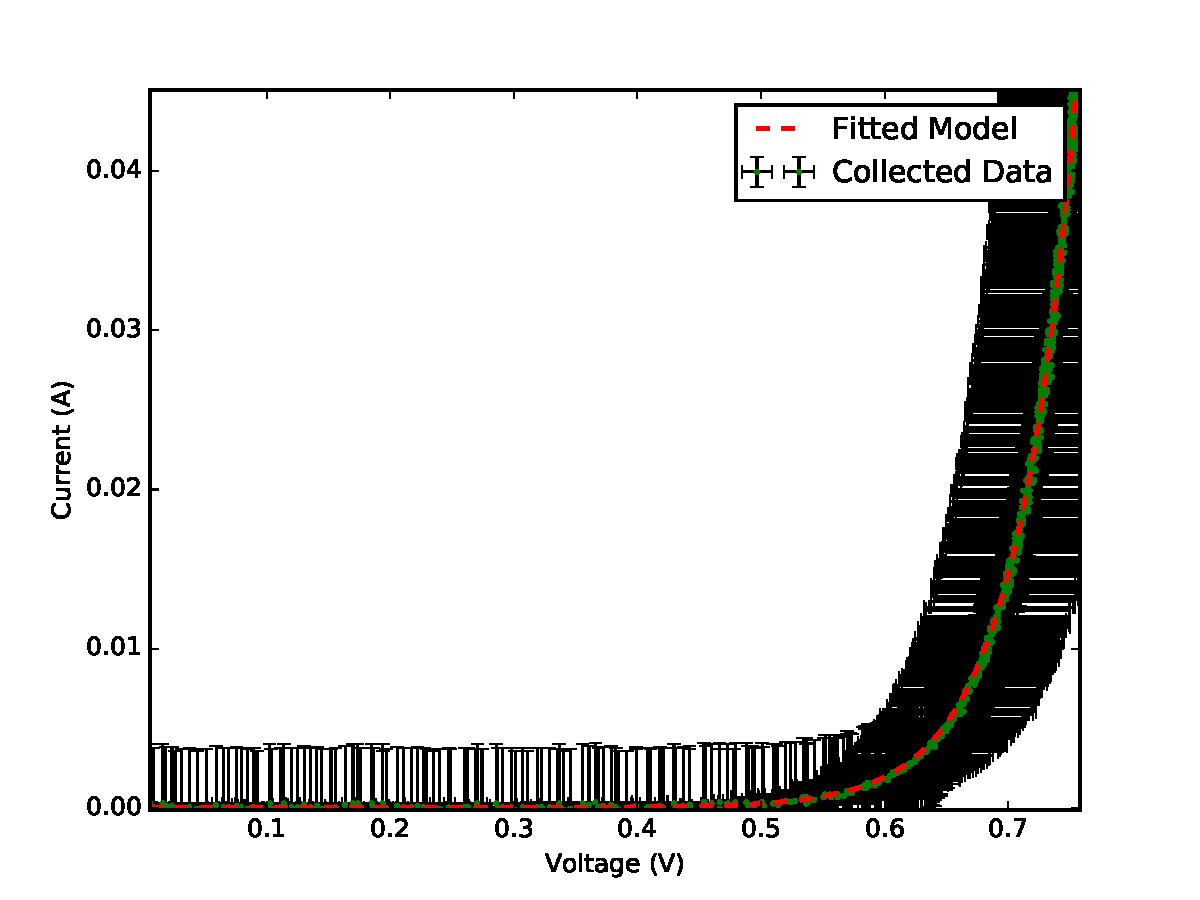
\includegraphics[width=\columnwidth]{../resources/plots/diode1_1n4001.pdf}
\caption{(Color Online) \textsc{1N4001} Data and Fit}
\label{fig:1N4001}
\end{figure}

\begin{figure}
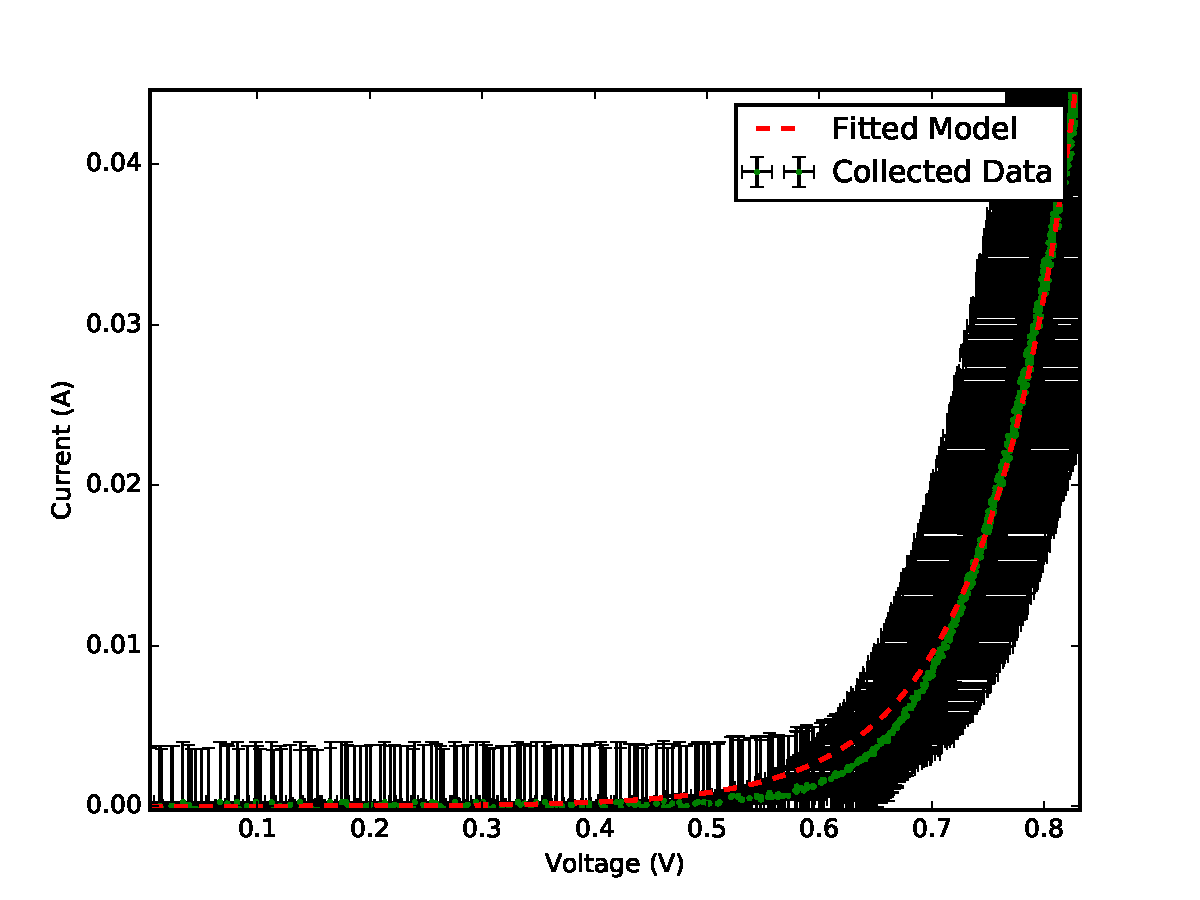
\includegraphics[width=\columnwidth]{../resources/plots/diode2_1n4148.pdf}
\caption{(Color Online) \textsc{1N4148} Data and Fit}
\label{fig:1N4148}
\end{figure}

\section{Discussion}

The low $\chi^2_{\rm{red}}$ indicate either an over-fitting of the data or an overestimation of the errors. The latter is likely the reason for the low values. As can be seen in \cref{fig:1N4001,fig:1N4148}, the error bars are quite large. The dominating term in \cref{eqn:sigma-current} is the $\sigma_V$ term, which is largely determined by the $58.4\:\rm{mV}$ input accuracy of the USB-6009. This is in fact the maximum variance cited by \cite{Instruments2014}; the typical operating accuracy is quoted at $4.28\:\rm{mV}$, which would significantly reduce the errors and improve the fit. Since we do not have the capability to measure the actual error of the USB-6009 and \cite{Instruments2014} does not specify the exact conditions of the different errors, results would not be credible without taking the maximum error.

\section{Conclusion}

In conclusion, it is obvious that this experiment has suffered from the large uncertainties involved. Following \cref{eqn:sigma-current}, $\sigma_I^2 \to 0$ as $R \to \infty$. However, it must also be realized that the current flowing through the circuit decreases as $R$ increases, as does the measurement error of the test resistor ($\sigma_R$) \cite{Keithley2003}. In future measurements of the IV curves, the value of $R$ should be carefully chosen so that $\sigma_I$ and $\sigma_R$ have optimal values.

The measurement could also be improved by minimizing $\sigma_V$ in \cref{eqn:sigma-current}. This can be done by either using a device that has lower error than the USB-6009 or by determining the conditions for the different errors given in \cite{Instruments2014} in order to obtain credible measurements at lower errors. The lab's Keithley 2700 voltmeter could be used to make all the measurements with improved accuracy and error at the expense of effort to either manually obtain data or interface with the Keithley's RS-232 port \cite{Keithley2003}.

An additional improvement that may be made in future experiments is careful attention to the fit model. \Cref{eqn:simple-fit} is known as the "ideal" diode equation, meaning that it does not perfectly account for the IV characteristic within a diode. Even with \cref{eqn:simple-fit}, there is a hidden dependence in $T$. The temperature is proportional to the velocity of atoms within the diode material. An exact dependence is dependent on characteristics of the diode material, which can vary from material to material and requires careful analysis and a loss of generality. Without a loss of generality, we can make a crude approximation by realizing that $I \propto v$ and $T \propto v^2$, leading to $T \propto I^2$. This results in a model of the form

\begin{equation}
I \mathrm{ln} I = \delta V 
\end{equation}

where $\delta$ is a constant. This equation has a solution of $I = e^{W\left(\delta V \right)}$ where $W$ is the Lambert W function \cite{lambertW}. The resulting model would be

\begin{equation}
I(V) = \eta e^{W \left(\delta V\right)}
\label{eqn:lambert-model}
\end{equation}

where $\eta$ and $\delta$ are fit parameters.

We attempted to fit the model given in \cref{eqn:lambert-model} for this failure, but were not successful. The use of the Lambert W function complicated the fitting of the model, which did not allow it to be fitted using the same methods as \cref{eqn:simple-fit} and thus is left to future work that can use a carefully-selected fitting method.


\bibliography{diode-characterization}

\end{document}